\section{Flüssigkristalle}

\subsection{Inhalt}
\begin{itemize}
\item Definition
\item  Atomarer Aufbau
\item flüssigkristalline Phasen
\item TN-Zellen
\end{itemize}

\subsection{Definition}

\subsection{Molekülstruktur}

\subsection{TN-Zelle (Twisted Nematic)}
\begin{minipage}{0.48\linewidth}
	\begin{center}
		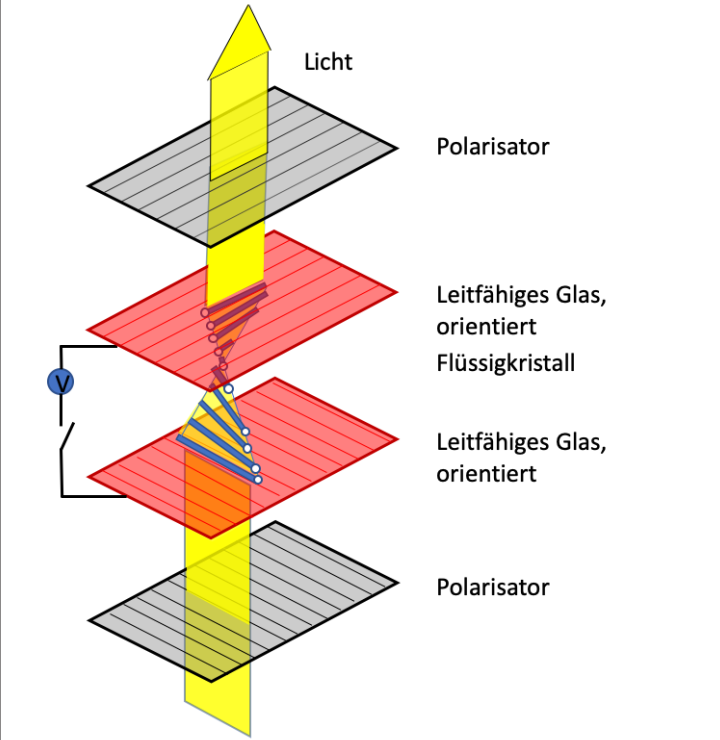
\includegraphics[width=0.8\linewidth]{images/TN-Zelle1.png}
		
		ohne angelegte Spannung   
	\end{center}
\end{minipage}
\hfill
\begin{minipage}{0.48\linewidth}
	\begin{center}
		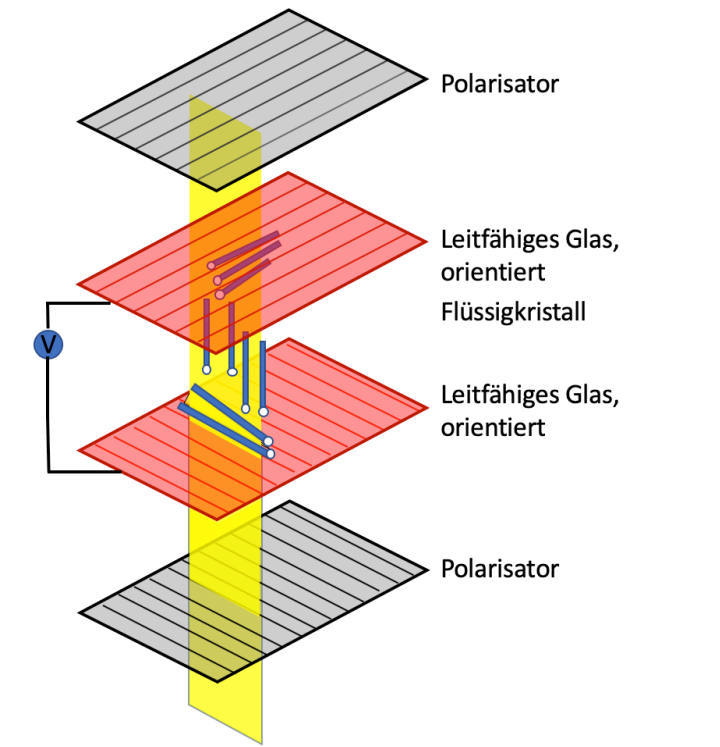
\includegraphics[width=0.8\linewidth]{images/TN-Zelle2.png} 
		
		mit angelegter Spannung 
	\end{center}
\end{minipage}
